\documentclass[10pt,a4paper,arial, spanish]{article}
\usepackage[spanish]{babel}
\usepackage[T1]{fontenc}
\usepackage[utf8]{inputenc}
\usepackage{listingsutf8}
\usepackage{graphicx}
\usepackage{float}
\usepackage{xcolor}
\usepackage[cache=false]{minted}
%\usemintedstyle{borland}
\usepackage[hidelinks, colorlinks=true, linkcolor=blue, urlcolor=blue]{hyperref}

\title{Proyecto Capstone - La Batalla de los Vecindarios (Semana 1)}
\author{R. Salaberry}
%\UseRawInputEncoding
\begin{document}



\maketitle

\begin{abstract}
	Como parte del curso IBM Data Science professional program Capstone Project, trabajaremos con un conjunto de datos reales con el fin de llevar a cabo un proyecto que abarque todas las instancias en las que un científico de datos se encontraría en la vida real al resolver un problema dado.
	
	El principal objetivo de este proyecto es utilizar todas las herramientas vistas en los cursos previos para la resolución de un problema de negocios dado, tal como lo haría en la vida real un científico de datos. 
	
	Se aplicarán los conocimientos adquiridos en la búsqueda de datos, la preparación de los mismos, el análisis y las conclusiones que implican para el caso de negocios planteado.
	El caso de negocio será la apertura de un restaurante de comida sudamericana (cono sur, Argentina, Uruguay, Brasil, Chile y Paraguay) muy populares en la región y que se conocen con el nombre de parrillas o parilladas en la ciudad de Toronto, Canadá. 
	 
	
\end{abstract}


\tableofcontents
\section{Definición del problema}
\subsection{Planteo del problema}
Toronto, una ciudad muy cosmopolita,  es la capital de la provincia de Ontario en Canadá. La ciudad ha albergado tradicionalmente muchas corrientes migratorias que se han establecido con el tiempo en sus barrios, de modo tal que hoy en día existen entre sus barrios, algunos que hacen referencias a la diversidad de culturas de dicha ciudad, como ser Chinatown, Corso Italia, Greektown, Kensington Market, Koreatown, Little India, Little Italy, Little Jamaica y Little Portugal.

% TODO: \usepackage{graphicx} required

\begin{figure}[H]
	\centering
	
\includegraphics[width=10cm, height=7cm]{Toronto}
	\caption[Ciudad de Toronto]{Ciudad de Toronto, Canadá.}
	\label{fig:toronto}
\end{figure}


En este proyecto, seguiremos paso a paso el proceso para saber si es buena idea la decisión de abrir un restauran de estilo sudamericano en la ciudad de Toronto, cuales son los barrios mas indicados para ello, teniendo en cuenta la migración de origen sudamericano y también los ingresos para cada barrio a fin de  crear para el restauran una clientela con un perfil económico aceptable.

Tomamos como definición de restaurante sudamericano (parrilla o parrillada) aquel en donde se cocina la carne de res a las brasas de la leña en una parilla. La comida típica así definida se denomina asado.

\begin{figure}[h]
	\centering
	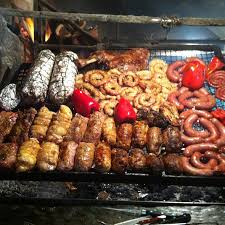
\includegraphics[width=10cm, height=7cm]{parrillada}
	\caption[Parrillada estilo sudamericano]{Parrillada estilo sudamericano}
	\label{fig:parrillada}
\end{figure}

Los países definidos como sudamericanos son los países pertenecientes al denominado cono sur, es decir Argentina, Uruguay, Brasil, Chile y Paraguay. Estos serán la población objetivo  a estudiar y relacionar con los barrios de Toronto.  

Para ello nos planteamos las siguientes preguntas:
\begin{itemize}
	\item  ¿En qué barrios de Toronto vive la comunidad sudamericana del cono sur? 
	\item  ¿Hay restaurantes de estilo sudamericano en Toronto, donde están ubicados? 
	\item  ¿Cómo es la distribución de ingresos de cada barrio de Toronto?
	\item  ¿Cuál es el barrio de Toronto mas apropiado para abrir un restaurante de estilo sudamericano (parrillada) ?  
\end{itemize}
\subsection{Perfil de interesados}
El perfil de personas interesadas en este problema son las personas relacionadas a la comunidad sudamericana de Toronto, y los empresarios sudamericanos que residiendo o no en Toronto deseen invertir en un restaurante típico en la ciudad, así como también cualquier empresario canadiense que quiera invertir en el rubro de gastronomía.

También representa interés a  la comunidad de científicos analistas de datos que deseen analizar los barrios de Toronto para un eventual modelo de negocio del rubro gastronómico.

\section{Fuente de datos. Adquisición y transformación}\label{datos}
Para este planteo vamos a precisar un detalle de los barrios de Toronto, que se puede obtener en Wikipedia desde el siguiente link: {\href{https://en.wikipedia.org/wiki/List_of_postal_codes_of_Canada:_M}{Datos código postal, barrios de Toronto}}. Tambien existe otra pagina con dicha información, es de {\href{https://www.zipcodesonline.com/2020/}{Zipcodesonline}} del año 2020 y tiene los zip codes de muchas ciudades del mundo, entre ellas los de Toronto en este link: {\href{https://www.zipcodesonline.com/2020/06/postal-code-of-toronto-in-2020.html}{Zip code de Toronto}} 

También el siguiente link de {\href{https://cocl.us/Geospatial_data\%E2\%80\%9D}{Coordenadas de códigos postales de Toronto, Canadá}} que proporciona la latitud y longitud de cada uno de los códigos postales que aparecen en la página de wikipedia anterior.

Finalmente vamos a necesitar información demográfica de los barrios de Toronto, esta información la obtenemos del portal de datos de la ciudad de Toronto, {\href{https://open.toronto.ca/dataset/neighbourhood-profiles/}{Datos de perfiles de barrios de Toronto, Canadá}}.

Para obtener la información sobre restaurantes en cada barrio de Toronto, usaremos la API de  {\href{https://developer.foursquare.com/docs}{Foursquare}}. Usando la API obtendremos los nombres, categorías, latitud y longitud de cada restauran existente en cada barrio de Toronto. En esta búsqueda se tratará de ubicar los restaurantes que cumplen con la definición de parrillas o parrilladas de estilo sudamericano.   

\section{Metodología}
Se trabaja con un Notebook Jupyter, realizando el código Python con un kernel Python 3.0.
Los pasos a seguir serán los siguientes:
\begin{itemize}
	\item Pasar a un data frame los datos de los barrios de Toronto de la página de wikipedia.
	\item Relacionar el data frame con las coordenadas latitud y longitud de archivo de coordenadas geográficas trabajado anteriormente.
	\item Obtener la información demográfica relevante de los barrios de Toronto y de la población emigrante de Sudamérica  desde  la base de datos del portal de datos de la ciudad de Toronto.
	\item Combinar los datos demográficos con la base anterior.
	\item Realizar el análisis de los datos para saber donde se ubica la población objetivo.
	\item Obtener datos de restaurantes relacionados (parrilladas) en los barrios de Toronto mediante consultas con la API de Foursquare.
	\item Relacionar la ubicación de dichos restaurantes con la ubicación de la población objetivo.
	\item Analizar los resultados obtenidos y realizar las recomendaciones necesarias.   
\end{itemize}


\end{document}
